% [Tamaño principal de la fuente del documento, tamaño del papel, con título (crea salto de página)]{Tipo de documento}
\documentclass[12pt, a4paper, titlepage]{article}
\usepackage[utf8]{inputenc}
% Traduce expresiones al español
\usepackage[spanish]{babel}
\usepackage{setspace}

\usepackage{graphicx}
\usepackage{geometry}
\geometry{margin=2.5cm}
\graphicspath{ {./imagenes/} }

% Permite utilizar labeling para listar de forma personalizada
\usepackage{scrextend}
% Permite centrar verticalmente m{}
\usepackage{array}

\title{\LARGE \textbf{Documentación de Proyecto - Cafetería Plus} \\[2ex] \Large Programación de Servicios y Procesos}
\author{\\[20ex]Cristian Fernández}
\date{\today}

\begin{document}
\maketitle

\doublespacing
\tableofcontents % Índice
\newpage

\section{Descripción del problema}
\noindent \\En esta ocasión recuperamos el proyecto anterior en el que simulábamos el funcionamiento de una cafetería mediante distintos hilos de ejecución con objeto de
expandir su funcionalidad mediante la implementación de una capa extra de complejidad, gracias a la cual seguiremos profundizando en el estudio de la sincronía de procesos. \\
Los puntos clave que nos permitirán dicha tarea serán la incorporación de los \textbf{métodos synchronized} junto con el uso del \textbf{patrón de diseño Productor/Consumidor}. \\ \\
El programa debe seguir estas pautas:\\
\begin{itemize}
    \item Crear una clase Barista (Productor).
    \item Crear dos clases Camarero (Consumidor).
    \item Crear una clase Cafetera (Búfer Compartido).
    \item Crear clases Cliente mediante la pulsación del botón \textit{`Dar Paso'}.
    \item Cada cliente debe intentar pedir un café y esperar el tiempo especificado. Los camareros deben esperar a que haya cafés disponibles y si es así servirlos en orden de
    llegada de la clientela. El barista debe hacer cafés incansablemente hasta que la cafetera no admita más (búfer lleno).
    Si un cliente se va antes de que su café esté listo, el camarero debe continuar con el siguiente cliente.
    \item El programa debe continuar ejecutándose hasta que se pulse el botón \textit{`Finalizar'}.
\end{itemize}
\newpage

\section{Patrón de diseño Productor/Consumidor}
\noindent \\El patrón de diseño Productor/Consumidor desacopla los procesos que producen datos de aquellos que los consumen, utilizando un búfer compartido para almacenar 
datos temporalmente. Este patrón es ideal para aplicaciones con tareas asincrónicas e independientes que se ejecutan a diferentes velocidades, mejorando la
escalabilidad y el rendimiento al permitir que el productor y el consumidor trabajen en paralelo. \\ \\
Sus componentes clave son:\\
\begin{itemize}
    \item \textbf{Productor}: Es un hilo o proceso que genera datos y los añade a una estructura de datos compartida, como una cola o búfer.
    \item \textbf{Consumidor}: Es un hilo o proceso que retira los datos del búfer y los procesa.
    \item \textbf{Búfer Compartido}: Es una estructura de datos (ej. una cola) que actúa como intermediario, almacenando los datos hasta que el consumidor esté listo para procesarlos.
    \item \textbf{Sincronización}: Mecanismos para controlar el acceso al búfer y asegurar que los productores no añadan datos a un búfer lleno y los consumidores no intenten retirar datos de un búfer vacío.
\end{itemize}
\newpage

\section{Nuevas clases}
\noindent \\A continuación unas capturas de las nuevas clases incorporadas al proyecto.\\\\
\begin{figure}[hbt!]
    \centering
    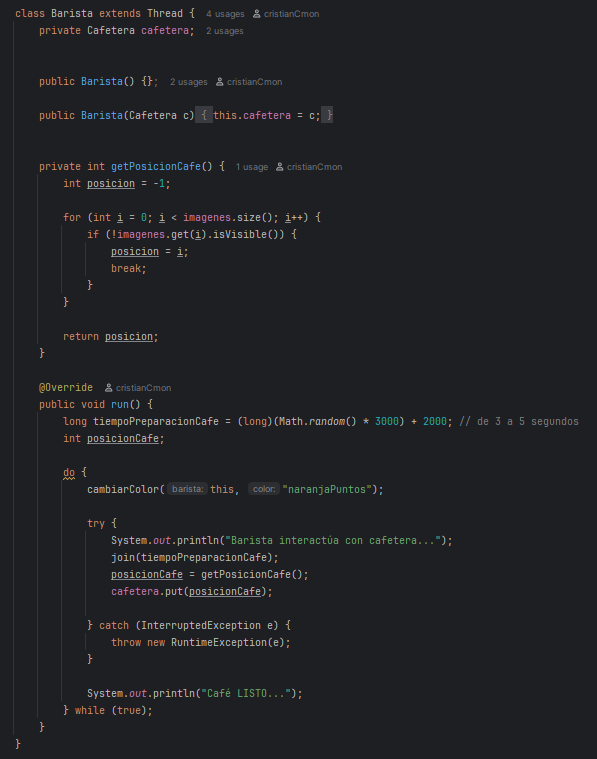
\includegraphics[width=0.8\textwidth]{barista.png}
    \caption{Clase Barista}
\end{figure}
\newpage
\begin{figure}[hbt!]
    \centering
    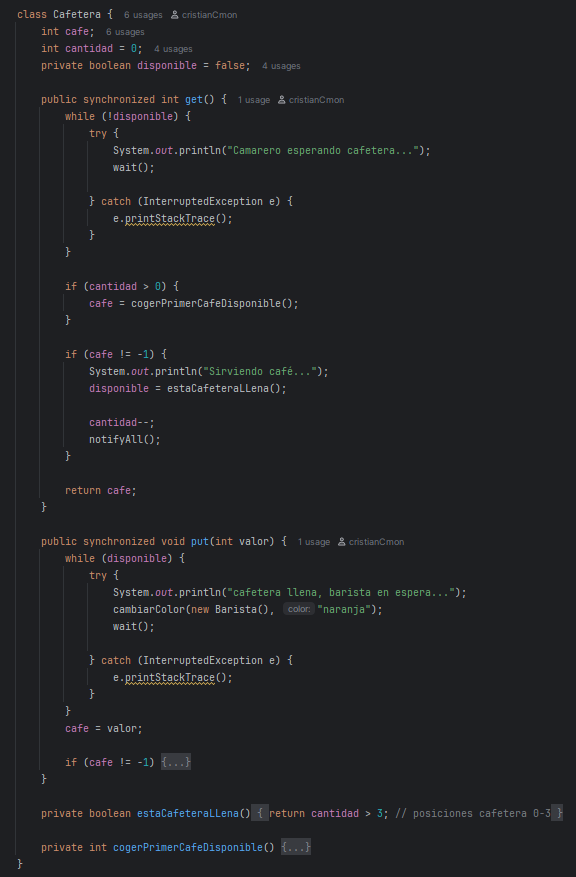
\includegraphics[width=0.8\textwidth]{cafetera.png}
    \caption{Clase Cafetera}
\end{figure}
\newpage

\section{Requisitos funcionales}
\noindent \\A continuación se listan los requisitos funcionales del sistema:\\
%\begin{description} sería equivalente pero items en negrita por defecto
\begin{labeling}{ RF-5:} % el segundo parámetro marca el espaciado entre ítem y texto
    \item[ \textbf{ RF-1}:] Ver una leyenda de colores que informen del estado de los Hilos.
    \item[ \textbf{ RF-2}:] Pulsar un botón que inicie la ejecución del programa.
    \item[ \textbf{ RF-3}:] Mostrar dinámicamente todo el proceso de ejecución.
    \item[ \textbf{ RF-4}:] Pulsar un botón que finalice la ejecución del programa.
\end{labeling}
\newpage

\section{Requisitos no funcionales}
\noindent \\A continuación se listan los requisitos NO funcionales del sistema:\\
\begin{labeling}{ RNF-5:}
    \item[ \textbf{RNF-1}:] El tiempo de respuesta al pulsar el botón Iniciar no debe superar los 2 segundos.
    \item[ \textbf{RNF-2}:] La intefaz gráfica de usuario ha de ser fácilmente entendible.
    \item[ \textbf{RNF-3}:] Cada acción realizada por los hilos debe ser lo suficientemente descriptiva para el usuario.
\end{labeling}
\newpage

\section{Casos de uso}
\noindent \\A continuación se muestran los casos de uso mediante la siguiente tabla:\\ \\ \\
\begin{tabular}{| m{5cm} | m{8cm} |} % | pinta las columnas verticales
\hline % pinta las filas horizontales
\textbf{Caso de uso} & \textbf{Descripción} \\
\hline
Consultar leyenda colores & El usuario consulta el funcionamiento de los hilos de la aplicación. \\
\hline
Iniciar aplicación & El usuario puede iniciar la aplicación pulsando un botón. \\
\hline
Terminar aplicación & El usuario puede finalizar la ejecución pulsando un botón. \\
\hline
\end{tabular}
\newpage

\section{Historias de usuario}
\noindent \\A continuación se muestran las historias de usuario mediante la siguiente tabla:\\ \\ \\
\begin{tabular}{| m{2cm} | m{2cm} | m{4cm} | m{4cm} |}
\hline
\textbf{ID} & \textbf{Como...} & \textbf{Quiero...} & \textbf{Para...} \\
\hline
HU-01 & Usuario & Pulsar un botón & Iniciar la aplicación \\
\hline
HU-02 & Usuario & Entender el comportamiento de los hilos & Deducir cómo funciona la concurrencia \\
\hline
HU-03 & Usuario & Pulsar un botón & Finalizar la ejecución de la aplicación \\
\hline
\end{tabular}
\newpage

\section{Herramientas de desarrollo}
\noindent \\
\begin{figure}[hbt!]
    \centering
    
\includegraphics[width=0.3\textwidth]{intellij.png}
\end{figure}
\noindent \\\textbf{IntelliJ Community Edition} es un IDE gratuito y de código abierto, ideal para el desarrollo en lenguajes JVM y Android.
Sus características principales incluyen un potente editor de código con autocompletado inteligente y refactorización, soporte para control de versiones, 
un depurador integrado, y herramientas de pruebas unitarias. Está disponible para todas las plataformas.  \\
\\Características principales: \\
\begin{itemize}
    \item \textbf{Editor de código potente:} Ofrece resaltado de sintaxis, análisis en tiempo real, sugerencias de código, e inspecciones y correcciones rápidas.
    \item \textbf{Soporte para múltiples lenguajes:} Es compatible con Java, Kotlin, Groovy, Scala, y otros lenguajes JVM.
    \item \textbf{Integración con control de versiones:} Permite la integración con sistemas como Git, SVN, y Mercurial.
\end{itemize}
\newpage

\section{Lenguajes de programación}
\noindent \\
\begin{figure}[hbt!]
    \centering
    
\includegraphics[width=0.6\textwidth]{javafx.jpg}
\end{figure}
\noindent \\\textbf{JavaFX} se caracteriza por su capacidad de crear aplicaciones enriquecidas visualmente, integrando multimedia (audio, video) y gráficos vectoriales.
Permite desarrollar aplicaciones multiplataforma (escritorio, web, móvil, smart TV). Otras características clave son 
la integración fluida con el ecosistema Java y herramientas como FXML y Scene Builder para un desarrollo más eficiente y colaborativo. \\
\\Características principales: \\
\begin{itemize}
    \item \textbf{Interfaces gráficas de usuario (GUI) enriquecidas:} Permite crear interfaces modernas y atractivas con animaciones, gráficos vectoriales, y elementos personalizables.
    \item \textbf{Integración multimedia:} Facilita la inclusión de contenido de audio, video y otros medios dentro de las aplicaciones.
    \item \textbf{Desarrollo declarativo (FXML):} Utiliza FXML, un lenguaje basado en XML, para describir la interfaz de usuario, lo que facilita el trabajo colaborativo entre diseñadores y desarrolladores.
\end{itemize}
\newpage

\section{Interfaz de la aplicación}
\noindent \\A continuación unas capturas de las diferentes vistas de la interfaz.\\\\
\begin{figure}[hbt!]
    \centering
    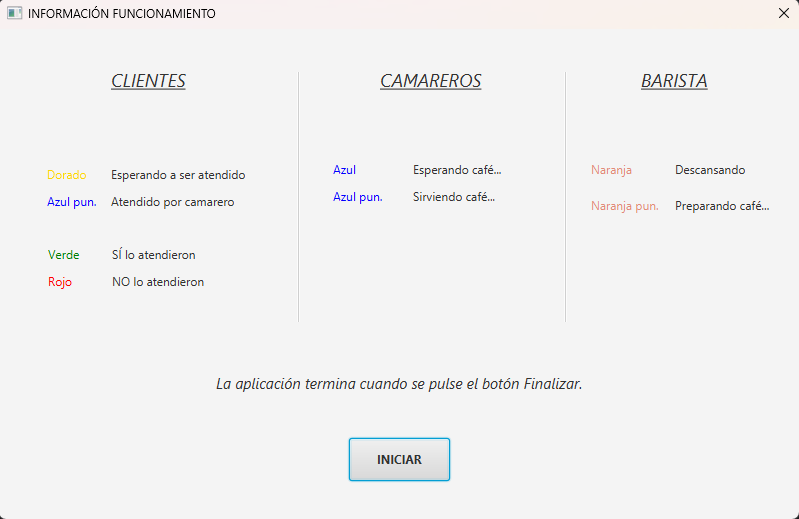
\includegraphics[width=1\textwidth]{captura0.png}
    \caption{Vista inicial, muestra comportamiento hilos por código de colores}
\end{figure}
\newpage
\begin{figure}[hbt!]
    \centering
    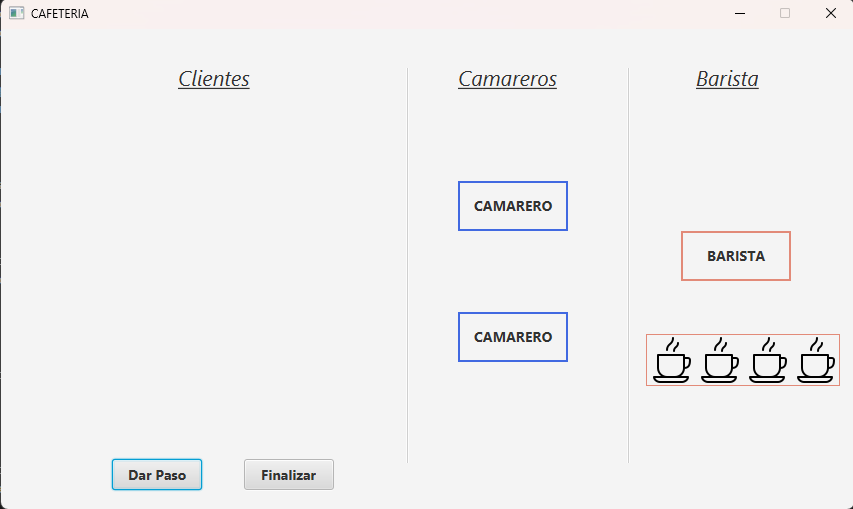
\includegraphics[width=1\textwidth]{captura1.png}
    \caption{Cafetera cargada y barista/camareros libres}
\end{figure}
\noindent \\
\begin{figure}[hbt!]
    \centering
    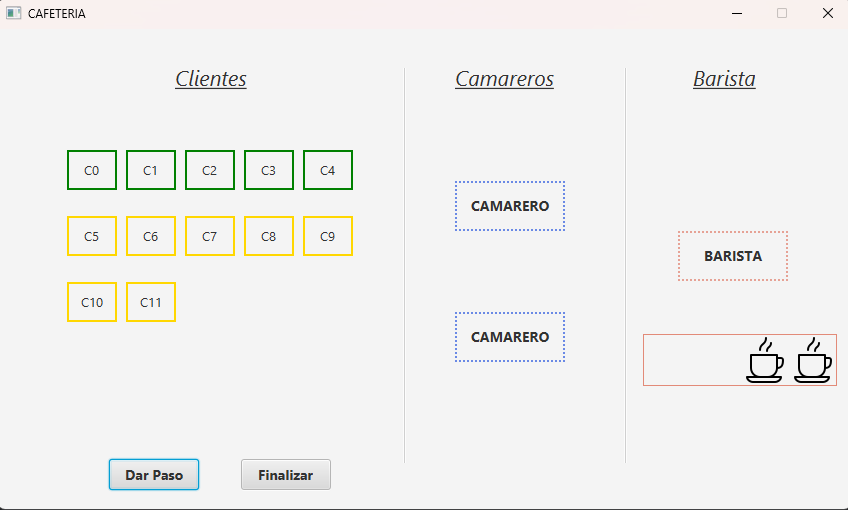
\includegraphics[width=1\textwidth]{captura2.png}
    \caption{Servicio normal con carga de trabajo rutinaria}
\end{figure}


\end{document}